\documentclass[11pt, a4paper]{article}
\usepackage[nochapters]{classicthesis}                              % template
\usepackage[margin=42mm]{geometry}                                  % margins
\usepackage[utf8]{inputenc}                                         % allow utf-8 input
\usepackage[T1]{fontenc}                                            % use 8-bit T1 fonts
\usepackage{graphicx}                                               % images
\usepackage{url}                                                    % URL typesetting
\usepackage{booktabs}                                               % good-looking tables
\usepackage{multirow}                                               % for tables
\usepackage{amsfonts}                                               % blackboard math symbols
\usepackage{amsmath}                                                % math ops
\usepackage{nicefrac}                                               % compact 1/2, etc.
\usepackage{microtype}                                              % microtypography

\definecolor{darkblue}{rgb}{0, 0, 0.5}                              % define link color
\hypersetup{colorlinks=true,citecolor=darkblue,                     % set link color
            linkcolor=darkblue, urlcolor=darkblue}

% Your packages here
% \usepackage{...}                                                  % some info, maybe

% !!! PLEASE CHANGE THESE VARIABLES TO MATCH YOUR INFORMATION !!!

\def\thesistitle{Measuring Domain-Specific Sentiment}                      % title
\def\subtitle{The WallStreetBets 'Meme-Stock' Saga}             % subtitle
    % ^if there is no subtitle, replace by \def\subtitle{}  
\def\yourname{Stefan Winter}                                                                       % ^first and last name
\def\yourprogramme{Data Science \& Society}                         % OR (remove this)
% \def\yourprogramme{Cognitive Science \& Artificial Intelligence}    % uncomment this
\def\yourstudentnumber{2067606}                                      % ANR (or u-number)
\def\finalmonth{January}
\def\finalyear{2022}
\def\supervisor{Dr. Peter Hendrix}
\def\committee{Dr. Raquel Garrido Alhama}
\def\acknowledgments{I want to thank Dr. Peter Hendrix for his invaluable guidance during this thesis.\\
Additionally, I want to thank Sveva Cadura and Anna Carolina van Melis for \\their support during the writing process.}

% METADATA

\hypersetup{pdfauthor   = \yourname,
            pdftitle    = \thesistitle\ \subtitle,
            pdfsubject  = \yourprogramme\ Master Thesis
}

% CHOOSE EITHER OF -----------------------------------------
% IEEE STYLE:

% \usepackage[square,numbers]{natbib}                               % bracket-style refs
% \usepackage{natbib}                                               % OR: parenthesized refs
% \bibliographystyle{IEEEtranN}

% OR -------------------

\usepackage[natbibapa]{apacite}                                     % only parentheses
\bibliographystyle{apacite}                                         % 'cause APA

% !!! ------------------------------------------------------ !!!

\begin{document}
% DON'T TOUCH THIS FILE, THANKS!

\pagenumbering{gobble}
\thispagestyle{empty}

\newgeometry{margin=30mm}
\begin{center}
\hspace{0.75cm}
\includegraphics[scale=0.5]{logo.eps} \\
\vspace{5cm}
\huge\spacedallcaps{\thesistitle} \\ [0.5cm]
\Large\spacedallcaps{\subtitle} \\ [1.2cm]
\normalsize\spacedallcaps{\yourname{}} \\ [1cm]
\normalsize{\spacedlowsmallcaps{Thesis submitted in partial fulfillment}} \\
\normalsize{\spacedlowsmallcaps{of the requirements for the degree of}} \\
\normalsize{\spacedlowsmallcaps{Master of Science in \yourprogramme{}}}\\
\normalsize{\spacedlowsmallcaps{at the School of Humanities and Digital Sciences}} \\
\normalsize{\spacedlowsmallcaps{of Tilburg University}} \\ [1.5cm]
\end{center}
\restoregeometry

\newpage

\begin{tabular}{l}
\noindent \spacedlowsmallcaps{student number} \\ [0.2cm]
\yourstudentnumber \\ [0.5cm]
\spacedlowsmallcaps{Committee} \\ [0.2cm]
\supervisor \\
\committee\\ [0.5cm]
\spacedlowsmallcaps{location} \\ [0.2cm]
Tilburg University    \\                        
School of Humanities and Digital Sciences \\
Department of Cognitive Science \& \\
Artificial Intelligence \\
Tilburg, The Netherlands \\ [0.5cm]
\spacedlowsmallcaps{date} \\ [0.2cm]
\today \\ \\
\spacedlowsmallcaps{Word Count} \\ [0.2cm]
8700 words
\end{tabular}
\vfill
\begin{tabular}{l}
\spacedlowsmallcaps{acknowledgments} \\ [0.2cm]
\noindent \acknowledgments{} \\ \\
\end{tabular}

\newpage

\newpage \pagenumbering{arabic}

\title{\rmfamily\normalfont\spacedallcaps{\thesistitle}\\[0.2cm]
       \rmfamily\small\spacedallcaps{\subtitle}}
\author{\spacedlowsmallcaps{\yourname}}
\date{}

\maketitle  % don't remove this :)

% --- start writing below:

\begin{abstract}
    Until the GameStop short-squeeze in early 2021, the impact of changes in sentiment of the Reddit discussion board \emph{WallStreetBets} on the financial market 
    was vastly underappreciated. Due to the novelty of this phenomenon, there is also almost no research available on that topic. This thesis will explore methodologies 
    on how to measure sentiment of the discussion board. One of the challenges when measuring the sentiment of WallStreetBets is the usage of novel 
    domain-specific words and terminologies, which are shown to have a big impact on the results of sentiment analysis. Hence, this thesis proposes a method 
    to create a dataset that covers the sentiment of text data which includes the terminology of a given domain. It will be shown that sentiment analysis machine 
    learning models that use the domain-specific text corpus as input outperform general purpose lexicons, which are currently commonly used by both academia and industry 
    to measure the sentiment of WallStreetBets.
\end{abstract}

\section{Introduction} \label{sec:introduction}

Modern society has been able to access vast amounts of information, communicate ideas, and become part of communities with the advent of the internet. 
Online discussion boards are playing a critical role by providing a platform where people can do so. Those discussion boards are also used by a 
variety of people to talk about the stock market and discuss trading strategies. Recently, the Reddit forum WallStreetBets has become one of 
the most well-known and influential investing online-forums.

Even though the Reddit subforum was created in 2012 already, it received the majority of its media exposure in 2021 as a result of a short-squeeze 
of the GameStop (GME) stock, which drove the stock price up hundreds of percentage points \citep{diangson2021betonreddit}. Over the ensuing months, however, 
the stock price experienced extraordinary volatility. Prices fluctuated by double-digit percentage points which not only lead to gains, but also to large losses
for market participants. Research shows that changes in investor sentiment and discussion board activity can be one cause of increased volatility \citep{das2007yahoo}.

However, it was not the rapid price appreciation in the beginning of the short-squeeze and volatility of the Gamestop stock that amazed market obervers. 
Instead, it was the unprecedented decentralized and coordinated buying of Gamestop shares by members of the WallStreetBets 
community that attracted attention \citep{anand2021WallstreetbetsAgainstWallstreet}.
Organizing the mass-coordinated buying of stock, however, requires that enough participants share the same sentiment. According to studies, 
social media sentiment has a particularly strong impact on uninformed traders \citep{danbolt2015InvestorSentiment}. It is argued, that coordinated investments will also
occur in the future, mainly due to the influence of social media and other online platforms on our society today \citep{semenova2021reddits}.
\\
Interestingly, finance scholars did not consider Reddit as a platform capable of having such a significant impact on the financial markets. 
As a result, the site has been neglected in their research \citep{long2021LikeTheStock}. \\*

\noindent
Hence, this thesis will try to answer the following Research Question:
\begin{quote}
\emph{How can sentiment analysis be performed on the WallStreetBets Reddit-forum?}
\end{quote}

To begin, it must be determined how the discussions about the Gamestop stock on WallStreetBets should be handled to serve as good input features for sentiment analysis. 
One of the challenges is the heavy use of peculiar terminology and domain-specific phrases on the WallStreetBets forum, as well as many novel words \citep{anand2021WallstreetbetsAgainstWallstreet}. 
According to recent research, sentiment lexicons and text-corpora with a focus on a certain domain produce superior sentiment analysis results compared to a 
general-purpose sentiment lexicon or text-corpus \citep{park2015EfficientExtraction}. Furthermore, the text data needs to be cleaned and pre-processed in order to be accurately 
processed by a machine learning algorithm \citep{jemai2021SentimentAnalysis}. As a result, the following sub-research question was formed:

\begin{itemize}
    \item[RQ1] \emph{How can the domain-specific language of the Reddit forum WallStreetBets be incorporated into sentiment analysis?}
\end{itemize}

Subsequently, machine learning models can be trained to perform sentiment analysis. However, 
each machine learning algorithm has its own idiosyncrasies and assumptions, and no single classifier 
works optimally in all possible scenarios. Hence, it is a good idea to evaluate the results and 
performance of different machine learning algorithms. As a result, the best model with a given set 
of hyperparameters can be selected to solve a particular problem \citep[p. 53]{raschka2019pythonmachinelearning}. 

This thesis will explore traditional machine learning methods such as Naive Bayes (NB) 
and Support Vector Machines (SVMs), as well as deep learning methods like 
Long Short Term Memory (LSTM) and Bidirectional Encoder Representations from 
Transformers (BERT). Due to the high dimensionality of textual data, deep learning methods have shown 
to outperform traditional machine learning techniques. That can be explained by the 
ability of deep learning methods to automatically learn the most important features, whereas traditional 
methods may suffer from the curse of dimensionality \citep{fu2018lexiconenhancedlstm}.
As was mentioned earlier, however, no classifier works best in all scenarios which is why the next sub-research question needs to be answered:

\begin{itemize}
    \item[RQ2] \emph{How do different sentiment analysis approaches perform based on the predefined evaluation metrics Accuracy, Precision, Recall and F$_1$-Score?}
\end{itemize}

\section{Related Work}

Gauging sentiment of online forums to predict movements in stock prices has been a research subject for many years now. 
\cite{das2007yahoo} did a study on the Yahoo! message board, which was amongst the first ones on the internet for investors to exchange ideas. 
\cite{lyocsa2021yolotrading} also showcased that as the discussion volume on WallStreetBets increased, the volatility of certain stocks got amplified. 
Additionally, the research of \cite{umar2021ataleofcompanyfundamentals} also found that sentiment of investors on WallStreetBets affected the returns of the Gamestop stock. 
However, they also demonstrate that other features such as the put-call ratio and the short-sale volume had a strong impact on the stock price. \\
\cite{long2021LikeTheStock} tried to uncover the impact of specific emotions such as \emph{“Angry, Fear, Happy, Sad and Surprise”} from the comments on 
WallStreetBets discussions on intraday changes of the stock price of the affected stock. While they conclude that the tone as well as the number of 
comments have an impact on the stock price, they show that the number of comments is not directly related to sentiment. Additionally, they argue it 
is the number of comments that is posted within an hour that has the biggest effect on 1-minute changes of the stock price. Furthermore, the paper 
shows that the emotions \emph{Sad, Angry and Surprise} have a significant impact on the gamestop 1-minute stock price. The Happy sentiment does not show a 
significant impact on 1-minute price changes, however, a causality test showed a link between the Happy sentiment and intraday returns of the GME stock. 
% In addition, the paper shows, that sentiment only impacts intraday returns if a thread has more than 2000 comments. // This does not fit well imo
Hence, the authors confirm that Reddit 
sentiment has an impact on the stock market. They also argue that any asset that is targeted by a large crowd from WallStreetBets can become a subject 
of excessive volatility, without being driven by any fundamental reasons.

However, since the WallStreetBets \emph{‘meme-stock movement’} is a relatively recent phenomenon, there is very little research on the impact of 
WallStreetBets on individual stocks, especially with regards to sentiment analysis. Additionally, of all the published research none account 
for the domain-specific language used on the forum. Because of the frequent usage of terminology that is specific to WallStreetBets, 
this can lead to incorrect conclusions.

Of course, this also applies to research in other fields, which usually also use a general-purpose sentiment lexicon, 
because of the cost associated with building a domain-specific one. However, it has been demonstrated that using a domain-specific 
knowledge base results in more accurate sentiment analysis results \citep{park2015EfficientExtraction}.
It is argued that there is no general-purpose sentiment lexicon that can be optimally applied on all domains. 
In different domains, some terms can have completely different meanings. A good example is the word “unpredictable”, 
which would have negative sentiment for electronics but can be a positive label for movies. It has been demonstrated 
that by adapting sentiment lexicons to a certain domain performance for sentiment classification can be enhanced 
\citep{Lu2011automaticconstruction}. This adapted lexicon can then be searched to find and score the sentiment 
of a specific word \citep{ashgar2014DetectionSlang}. 
While lexicon-based methods have found widespread adoption, mainly due to their simplicity, more advanced machine 
learning methods have also shown stronger performance \citep{wang2020automaticconstructiondomainsentiment}.

For this reason some research deviates from lexicon-based approaches. Instead, they examine how deep learning methods can be 
used to automatically detect and identify domain-specific words in sentences. By doing so it is assumed that the 
algorithm can not only detect whether domain-specific words are used (sentence-level detection), but also identify 
the exact position of the term in the sentence (token-level identification). Hence, it is possible to detect new meanings 
of words in an already existing text corpus. In addition, this approach also allows to classify novel words, that do not yet 
exist in a lexicon. This can be achieved by having models that formulate domain-specific word detection as a 
sequence-labelling task. Furthermore, novel domain-specific words can be learned by understanding the contextual 
structure of a sentence \citep{pei2019slang}. Those out-of-vocabulary tokens can be learned in the hidden layers of 
LSTMs \citep{hochreiter1997lstm}. To further optimize performance, models can be improved, by applying a character-based 
convolutional neural network to encode the spelling of words \citep{pei2019slang}. Other research shows that the accuracy of an
LSTM can be improved by introducing Word2Vec into pre-training the LSTM. As a result, the one-hot encoded input to the LSTM is
converted into a low dimensional vector that covers the semantic similarity of the words in it. Due to the lower dimensionality,
over fitting can be prevented and the network may also need less parameters \citep{xiao2018word2veclstm}.

Other research demonstrates the importance of large pre-trained models using transfer learning \citep{deng2009transferlearning}.
\cite{devlin2019bert} introduce BERT, a pre-trained model that uses the English Wikipedia and the BooksCorpus, which shows promising results.
One of the advantages is that only one output layer needs to be added to the model to achieve state-of-the-art sentiment analysis performance.
However, it is also shown that BERT lacks domain awareness. Hence it cannot differentiate between properties of source and target domains. One
proposed solution is to replace a random subset of tokens by a \emph{MASK} token. The corresponding hidden values of the MASK token can be fed
into the output layer. This adaption to a specific domain is shown to slightly enhance the performance of a vanilla implementation of BERT. However,
it is also argued that a vanilla implementation can still outperform other models \citep{Du2020AdversarialAD}.


Even though the literature suggests many 
innovative ways to enhance model performance by a few percentage points, the biggest benefits seem to come from high quality 
input data in the form of domain-specific labeled data.

Creating a domain-specific annotated corpus to train machine learning models, however, is not without its own challenges. 
For example, working with multiple human annotators can lead to discrepancies in the annotation results \citep{kim2008corpusannotation, rayan2019sentimentanalysisemail}. 
Additionally, it is hard to estimate the total annotation cost which can depend of various factors. One example would be whether the annotator is capable of fluently understanding 
the language for the given task \citep{arora2009estimationgannotationcost}. Additionally, labelling an entire dataset incurs extremely high costs, 
which can be avoided. With the support of an Active Learner, a complete domain-specific corpus with its respective labels can be 
created using only partial annotations \citep{park2015EfficientExtraction}. 

One of the key concepts of Active Learners is that if a machine learning algorithm is allowed to choose the data from which it learns, 
it will achieve higher accuracy with less training data. If a considerable amount of the data is unlabeled, this is especially desirable. 
As a result, the total cost of annotation can be reduced drastically. Research shows that the total number of 
manual annotations can be reduced by 80\% when using an Active Learner instead of randomly 
selecting data to label \citep{baldridgeosborne2004active}.

If data are manually annotated at random, the annotator will invest a lot of time into labeling irrelevant instances. 
This may incur costs which could be avoided with an Active Learner. It is argued that Passive Learning, or randomly selecting instances 
to be labeled by an annotator, is especially costly if the class distribution of the data is imbalanced or if there are many very similar documents. 
For example, if a specific feature set appears on only 1\% of instances, the annotator would have to label 1000 documents to cover 
the feature set on 10 relevant documents. When it comes to document similarity, large clusters of very similar documents might be 
identifiable. Because features may be barely distinctable, the annotator might spend a lot of effort labeling uninformative instances 
when selecting them randomly. An Active Learner, on the other hand, suggests which instances the annotator should label. Those instances can be 
determined on various quantitative metrics \citep{miller2020activelearningapproaches}.

\section{Method}

\subsection{Data} \label{subs:data}

While Reddit does offer an official API, the API is most useful for streaming data. 
There are some strict limitations on accessing large amounts of historical data. As a result, the official API is not the best choice for this thesis. 
However, \emph{pushshift.io} provides a solution for the strict limits.
The FAQ on the pushshift subreddit states, that pushshift data is best used to:
\begin{itemize}
    \item 'Analyze large quantities of Reddit data'
    \item 'Grab data for a specific date range in the past'
    \item 'Search for comments'
    \item 'Aggregate data'
\end{itemize}

Pushshift copies data from Reddit at the time it is posted. Since Pushshift uses the document-based database Elastic, it is extremely fast to query data \citep{elastic2015}. However, currently Pushshift does not regularly update certain metadata, such as scores, edits to a submission’s text or comments. Hence, there might be some minor inconsistencies of what is shown on Reddit and what is in the database. The scores, for example can easily be accessed via the official reddit API and, if needed, joined with the data obtained from Pushshift. Based on the data verification that was performed for this thesis, the number of comments only deviates by a marginally small amount. It is hypothesized that the small difference can be explained by forum moderators deleting spam. Those spam comments are assumed to not have a big impact the thesis anyways, which is why the small difference in the number of comments do not need to be addressed. \\
To access Pushshift, this thesis uses an API wrapper called \emph{PMAW}. Since requests are I/O-bound, PMAW is multithreaded. Hence requests can be run asynchronously which allows the data to be loaded much faster \citep{pmaw2021}.
When making the API request, the most important parameters are the following:
\begin{itemize}
    \item subreddit: Name of the subreddit
    \item q: The search term based on which the subreddit is queried
    \item before: The starting date of the query
    \item after: The end date of the query
\end{itemize}

For this thesis all Gamestop (GME) related posts between January 1st, 2020 and October 26th, 2021 were requested for the subreddit WallStreetBets. 
The query returns 89 columns. Most of which, however, can be dropped since they either aren’t useful for this thesis or contain no data. 
The most important columns are the number of comments, the title of the post and the content of the post. 
Emoticons are also included in the content text. In total 179,544 posts were obtained.\\
Of all obtained posts, 10\% or 17,955 were manually labeled as \emph{bearish, neutral or bullish}. Generally, bearish is associated with negative 
sentiment where investors assume a decline in stock prices. Bullish, on the other hand, relates to positive sentiment where investors hope for rising stock prices.

\subsection{Data Preprocessing} \label{subs:datapreprocessing}
The research by \cite{jemai2021SentimentAnalysis} presents a system for structuring a sentiment analysis project. 
The data collection phase is the first step, where textual data is obtained from a source. 
The data is then cleaned in the second step, the data pre-processing phase. To do so, several actions need to be performed.
One of them is tokenization. This is a natural language processing technique in which a large body of text is broken down into multiple sentences, 
each of which is then broken down into a list of words. Stop words such as is, the, a and other common words are also removed during the 
pre-processing phase. If stop words are included, they may play a negative role in sentiment classification and increase the overall 
vocabulary size while having little predictive power. \citep{zhao2017comparisontextprocess}.
In addition, special characters such as @ and urls should also be removed. 
It is also suggested that the text is converted to lowercase. As the final step, the research proposes lemmatization. By doing so,
the structure of a word is analyzed and converted to its normalized form. The research conducted by \cite{camachocollados2018role} 
shows that lemmatization improves sentiment analysis results when using domain-specific datasets.

Since it is shown that having data with emoticons leads to more accurate results than data without emoticons,
this thesis does not remove emoticons from the text corpus \citep{parveen2016sentimentanalysistwitter}.
Eventually, term frequency-inverse document frequency (tf-idf), was applied on the text corpus. 
Using this representation allows the extraction of the most descriptive terms in a document and easy computations. 
However, it fails to capture semantics and word embeddings. For computational reasons, only words that occur at least five times were included in the tf-idf representation. % Update this in the end when I know how much my computer can handle...

\subsection{The Case for a Semi-Supervised Method over an Unsupervised Method} \label{subs:supervisedvsunsupervised}
Since the data obtained from Reddit is unlabeled, it cannot be fed into supervised machine learning algorithms. 
That is because supervised sentiment analysis methods rely on labeled data \citep{sazzed2021ssentia}. One approach to label 
data is using unsupervised machine learning models. Unsupervised models are commonly applied in Natural Language Processing 
and text classification \citep{jung2019automatedclassification}. However, unsupervised models are a better choice for uncovering hidden 
patterns in a dataset, especially without any a priori knowledge of the structure of the data. As a result, unsupervised models 
excel at summarizing or exploration a large text corpus. 
For the case at hand, a t-Distributed Stochastic Neighbor embedding (t-sne) algorithm was applied on the data to extract similarity 
features and project them onto a lower dimension \citep{binu2020dimreductiontsne}. As can be seen in Figure 1, admittedly 
at a low dimension, the majority of the data do not belong to any particular cluster.

\begin{figure}
    \centering
    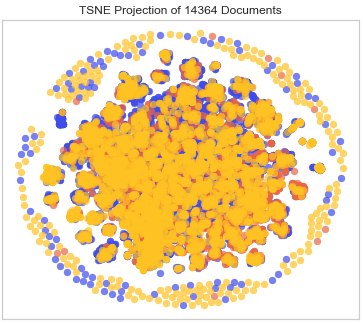
\includegraphics[width=\textwidth]{tsne_projection.png}
    \caption{t-sne visualization of seed data}
    \label{fig:t-sne}
\end{figure}

Even though there are some approaches to clustering high dimensional data, it generally is difficult to do so. 
One of the explanations for that is the increased sparsity and the difficulty to distinguish between the distances 
of specific instances \citep{tomasev2014roleofhubness}.

Once labeled instances are obtained, supervised learning methods can be applied.
One of the major disadvantages of supervised models, however, is the cost associated with manually labelling 
the data \citep{miller2020activelearningapproaches}.
This thesis proposes a method to create a labeled dataset for the fraction of the total annotation cost. 
As a result, a domain-specific labeled text corpus is created, which can be used to compare the performance of different supervised machine learning algorithms.
The proposed methodology is an Active Learner. With its support, a complete domain-specific corpus can be labeled while only relying on partial annotations \citep{park2015EfficientExtraction}. 

\subsection{Active Learner Workflow} \label{subs:activelearnerworkflow}
The illustrated workflow in Figure 2 provides an overview of how an Active Learner works. 
To begin with, cleaned and pre-processed data needs to be available that can be used by the Active Learner. 
Furthermore, the Active Learner can also be trained with some initial training data, which is also referred to as the seed. 
By using clustering algorithms, the seed data can be selected and labeled methodologically, which allows the Active Learner to achieve 
higher accuracy faster when compared to randomly picking the initial seed data \citep{kang2004usingclusterbasedsampling}. All the unlabeled 
instances will become the pool data, which need to be labeled. The seed data is fed into the Active Learner and trains an estimator, 
which needs to be defined when creating the Active Learner.\\
In addition, a query strategy needs to be defined, based on which the Active Learner queries new instances from the aforementioned pool. 
A query strategy evaluates the informativeness of unlabeled samples. Common strategies are \emph{uncertainty sampling, query-by-committee, 
expected model change, expected error reduction and variance reduction}. \\
While each strategy has its own intricacies, all essentially try to find instances that are hard for the model to classify and hence might benefit from manual annotation. 
After the query function selected instances from the pool, an oracle needs to label those. An oracle normally is at 
least one human with knowledge on how to annotate the data at hand \citep{settles2009activeLL}. Once the new instances are labeled, 
those instances need to be removed from the pool, since they are now part of the labeled data. The Active Learner then needs 
to be taught the new instances, which he can use to adjust the model. After each iteration, the results can be evaluated. 
A common performance measure for Active Learners is \emph{accuracy}.\\
If a predefined stopping criterion is not yet met, the query strategy selects more instances from the pool and repeats the process.
If the stopping criterion is met, the process ends \citep{lu2019investigating}.

\begin{figure}
    \centering
    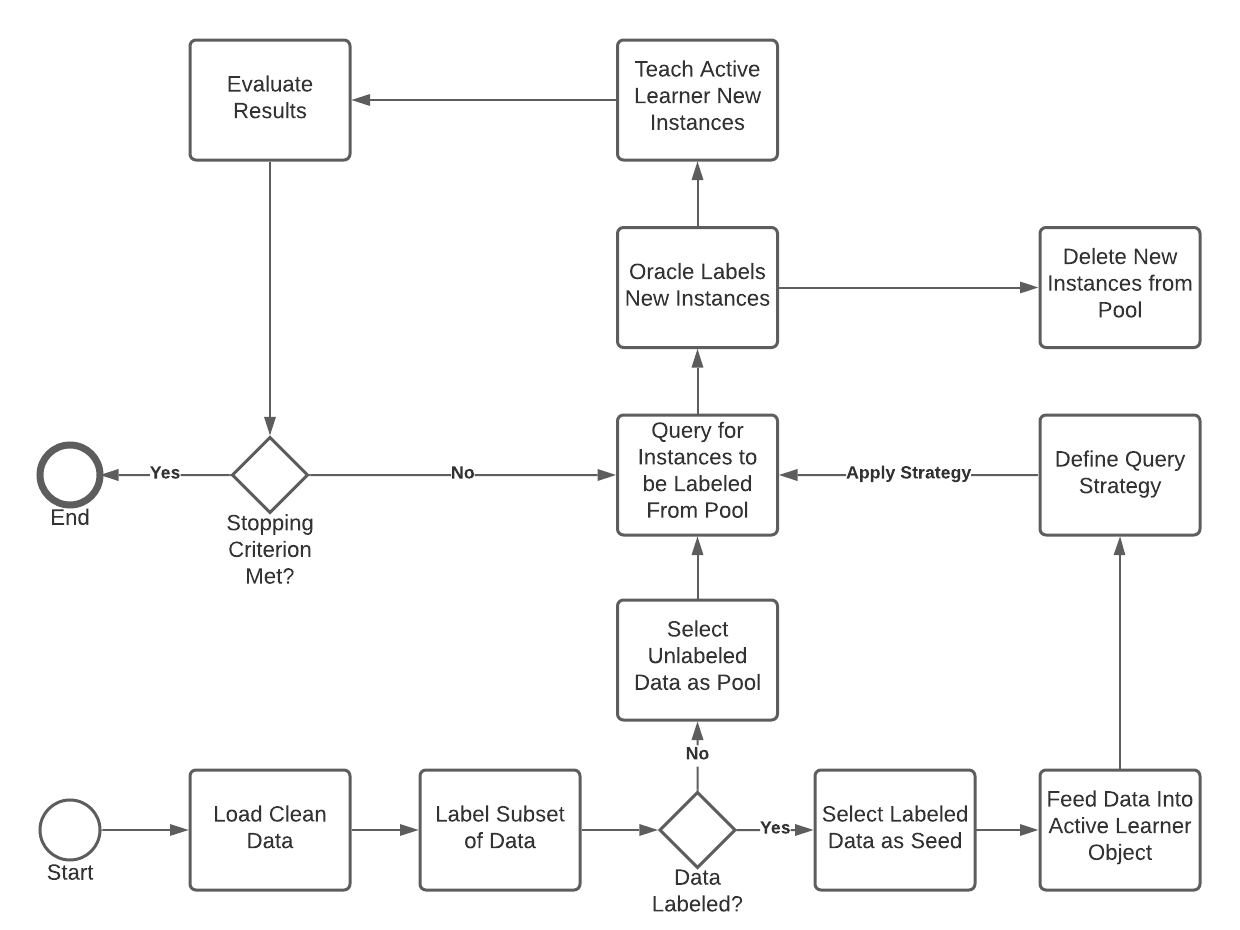
\includegraphics[width=\textwidth]{al_workflow.png}
    \caption{Visualized Workflow of an Active Learner. Created with lucid.app}
    \label{fig:AL_Workflow}
\end{figure}

\subsection{Active Learner Implementation} \label{subs:activelearnerimplementation}
To implement an Active Learner the \emph{modAL} package was used. modAL was designed with modularity, flexibility and extensibility as high priorities \citep{danka2018modal}. 
The estimator defined in the Active Learner object is a Support Vector Machine (SVM). A SVM was chosen because of its strong generalization 
performance \citep{alves2014comparisonsvm}.
Additionally, SVMs can be used to solve both regression and 
classification problems. For the case at hand, the algorithm needs solve a classification problem, by optimally separating the data between bearish, 
neutral and bullish instances. Classification is done by finding a hyper-plane with the biggest margin, meaning it looks for the greatest distance 
to the nearest sample points \citep{jemai2021SentimentAnalysis}. SVMs use spatial transformations, commonly known as kernel functions, to fit the hyperplane. 
Kernels can be linear, RBF or others. The radial basis function (RBF) kernel is best used for non-linear problems and is a general-purpose kernel that 
is often used in pattern recognition problems. The linear kernel, on the other hand, is typically used when there are only two classes present. 
A good example for that might be positive and negative sentiment \citep{alves2014comparisonsvm}.

The initial seed data to train the SVM-estimator in the Active Learner had to be labeled manually. To do so, every tenth instance was annotated.
Furthermore, the implementation of the Active Learner in this thesis deviates from the literature a little bit: The literature that was reviewed
does not set aside a test set from the initial seed data and the accuracy of the Active Learner is evaluated on the entire seed data after every iteration. 
While the literature does not explain why this approach was
taken, I hypothesize that is due to the cost associated with labeling the data. This thesis will not deviate from well established machine learning practices
and therefore set aside 20\% of the seed data as test data, which will be used to evaluate the performance of the Active Learner after every iteration. \emph{Insert citation from my ML book}

Uncertainty sampling was chosen as the query strategy because it has been demonstrated to be a strong baseline strategy. 
This query strategy assumes, that instances that are far from the decision boundary are adequately explainable and instances close to the 
decision boundary are uncertain. Naturally, this complements the SVM-estimator very well. As a result, the Active Learner queries 
the samples about which it is most uncertain about \citep{osbonre2004ensemblebased}.

\subsection{Sentiment Analysis Models} \label{subs:sentimentmodels}
The next section explores the machine learning models that will be used to perform sentiment analysis on the domain-specific corpus created by the Active Learner. \\
%Because a SVM was used in the Active Learner to label the ground truth data, it will not be applied in the sentiment classification task. 
%Otherwise, the results might lack robustness and be biased. \\
Before training the models, 20\% of the data were set aside as the test set. To account for class imbalances, stratification was applied.  

\subsubsection{Naïve Bayes (NB)} \label{subs:naivebayes}
NB is a probabilistic supervised machine learning model. By working probabilistically, the classifier assigns the probability of 
belonging to a given class based on certain features \citep{jemai2021SentimentAnalysis}. Because of the high dimensionality of textual data, 
which can be handled very well by NB, this algorithm has established itself as one of the standards for sentiment analysis. 
This thesis will use Multinomial Naïve Bayes to classify the sentiment of the text. This is due to the model’s ability to handle 
larger vocabulary sizes. In addition, the algorithm is simple to implement, suitable for real-time applications, and highly scalable. 
However, the algorithm’s prediction accuracy is frequently lower than that of other sentiment analysis techniques \citep{song2017novelclassification}. 
Due to the easy implementation and fast training of the algorithm, Naïve Bayes will serve as the baseline classifier.

\subsubsection{Long Short Term Memory (LSTM)} \label{subs:lstm}
LSTMs are becoming increasingly popular for sentiment classification. 
LSTMs are built on a recurrent neural network architecture (RNN). In an RNN the neurons are connected to themselves through time. 
As a result, the input from a time instance t\textsubscript{i} will also be used as an input for the next time instance t\textsubscript{i+1}.That leads to the 
problem of vanishing gradients, which means that it is hard for the model to learn long-term dependencies. This occurs because
in a long sequence, like a sentence, as the loss gradients are backpropagated through the RNN, they may shrink to zero \citep{vanishinggradients2020pmlr}.
LSTMS are designed to overcome that problem.
The LSTM architecture does so via its four constituents: A memory cell which can remember a lot of information 
from previous states, an input gate which controls the inputs into the neurons, an output gate with an activation function 
and lastly a forget gate which resets the neuron \citep{priyantina2019sentimentanalysishotel}. \\


\noindent\textbf{Implementation}\\
To feed the data into the LSTM, it first is converted from a tf-idf representation into a one-hot encoded array with three dimensions. However, one-hot encoding fails to incorporate similarity between words, which is why an Embedding layer was added to the LSTM. The layer takes the number of words in the text corpus as input. The output dimensions which will be used in the subsequent LSTM layer are a hyperparameter and chosen by evaluating the performance on the validation set, which is 20% of the training data. The same applies to the hidden states in the LSTM layer. The final Dense output layer uses softmax as its activation to output either bearish, neutral or bullish. Furthermore, the model uses categorical crossentropy as its cost function and accuracy as its metric. The optimizer is also chosen based on the hyperparameters provided.


\subsubsection{Bidirectional Encoder Representations from Transformers (BERT)} \label{subs:bert}
BERT is a relatively new machine learning algorithm developed by Google in 2018 and mainly designed for 
natural language processing. BERT is pretrained on the English Wikipedia and BooksCorpus. Because of the 
pretraining users won’t need as much computing power to achieve good results, even if the dataset is relatively 
small \citep{devlin2019bert}. The BERT github page even states that 
“Most NLP researchers will never need to pre-train their own model from scratch” \citep{googlegithub}

\subsection{Hyperparameter Tuning} \label{subs:hyperparams}
In order to find the best performing models, some hyperparameter tuning steps were taken. For the implementation of the Naïve model, five-fold grid search cross-validation was used to find the best parameters in a pre-defined parameter grid.
For the deep learning models, LSTM and BERT, a loop was created that iterates over a set of parameters. Within each iteration, the model is fit on the training data while setting aside 20\% of the data for validation. The best performing model
and its respective parameters will then be used to classify the test data. 

\subsection{Data, Code and Ethics Statements} \label{datacodeethics}
To query the data from pushshift, the explanation of pmaw API wrapper from Github was used: \url{https://github.com/mattpodolak/pmaw}\\
The data was manually verified, by comparing specific, randomly-sampled, instances with the actual posts on reddit.\\

\noindent To label the initial train set, I created a graphical user interface using tkinter: \url{https://docs.python.org/3/library/tkinter.html}\\

\noindent To create the t-sne visualization, I relied on the documentation provided by Yellowbrick: \url{https://www.scikit-yb.org/en/latest/api/text/tsne.html}\\

\noindent To implement the Active Learner, I used modAL: \url{https://github.com/modAL-python/modAL}\\

\noindent All scikit\-learn packages and classes, such as train\_test\_split, TfidfVecotricer, LabelEncoder, GridSearchCV, 
Pipeline, SVM and NB were implemented by utilizing material provided during the Machine Learning course at Tilburg University, taught by Dr. Güven and Dr. Önal.\\

\noindent The LSTM was implemented by using material provided during the Deep Learning course at Tilburg University, taught by Dr. Vanmassenhove and Dr. Saygili.\\

\noindent To implement BERT the following tutorial was used: \url{https://skimai.com/fine-tuning-bert-for-sentiment-analysis/}\\


\noindent The code for this thesis is shared in the following github repository: \url{https://github.com/StefanWinterToo/Master-Thesis}\\

\noindent All graphics used in this thesis were created by myself.\\

\noindent Due to time constraints, this first-submission does not use the full set of all possible hyperparameters and trains the LSTM and BERT only on a subset of the data.
Furthermore, for the Active Learner the VADER sentiment lexicon was used as an oracle.\\

\noindent To the best of my knowledge, the literature used was referenced appropriately.

\section{Results}

Figure 3 shows the accuracy of the Active Learner. As can be seen in the graph, the performance of the Active Learner slightly decreases over time.

\begin{figure}
    \centering
    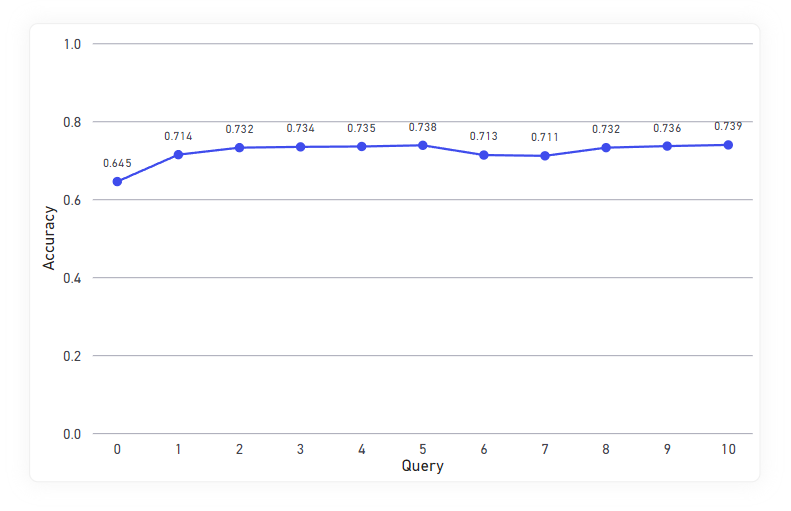
\includegraphics[width=\textwidth]{ActiveLearner.png}
    \caption{Accuracy of Active Learner over 20 iterations}
    \label{fig:ActiveLearner}
\end{figure}

The overview in Table 1 shows which sentiment classifier performed best. Both the LSTM and BERT fail to outperform the NB baseline model.

\begin{table}
    \caption{Test scores for NB, LSTM and BERT}
    \label{tab:results}
    \centering
    \small

    \begin{tabular}{lllrr}
        \toprule
                                        & \multicolumn{4}{c}{Evaluation Metrics} \\
                                        \cmidrule{2-5}
                            Model       & Accuracy      & Precision     & Recall    & F\textsubscript{1}-Score \\
            \midrule
            \multirow{1}{*}{NB}         & 0.79          & 0.74          & 0.82      & 0.76                      \\
            \midrule
            \multirow{1}{*}{LSTM}       & 0.00          & 0.53          & 0.53      & 0.53                      \\
            \midrule
            \multirow{1}{*}{BERT}       & 0.52          & 0.17          & 0.33      & 0.23                      \\

        \bottomrule
    \end{tabular}

\end{table}

The accuracy of the LSTM on the validation set is highest after 10 epochs, while the loss starts to increase by a lot. As a result, the weights and other parameters
seem to be optimal at epoch 10, which is why they will be used for the final model.
\begin{figure}
    \centering
    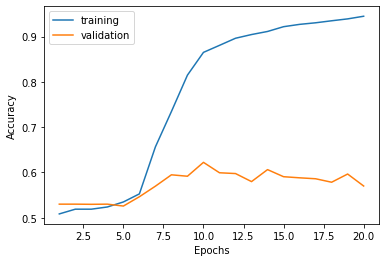
\includegraphics[width=\textwidth]{LSTM_acc.png}
    \caption{Accuracy of LSTM over epochs}
    \label{fig:LSTM_acc}
\end{figure}
\begin{figure}
    \centering
    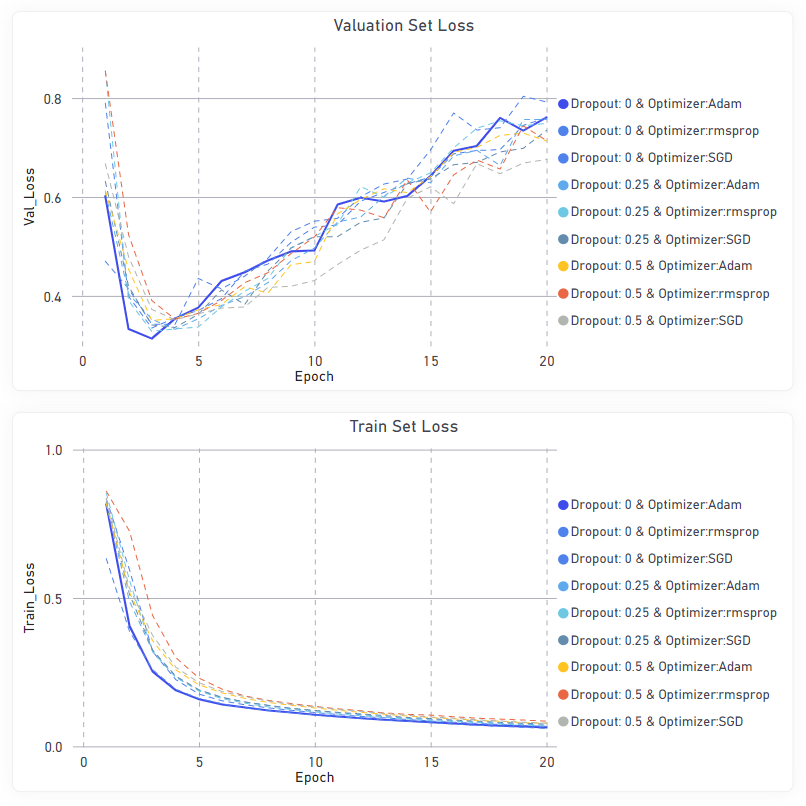
\includegraphics[width=\textwidth]{LSTM_Loss.png}
    \caption{Loss of LSTM over epochs}
    \label{fig:LSTM_Loss}
\end{figure}

Since BERT is already pre-trained, it does not need as many epochs to optimize a model. As can be seen in figure 5, there is almost no change to the accuracy.
However, the loss drops.

\begin{figure}
    \centering
    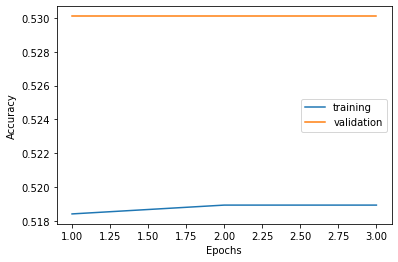
\includegraphics[width=\textwidth]{BERT_acc.png}
    \caption{Accuracy of LSTM over epochs}
    \label{fig:BERT_acc}
\end{figure}
\begin{figure}
    \centering
    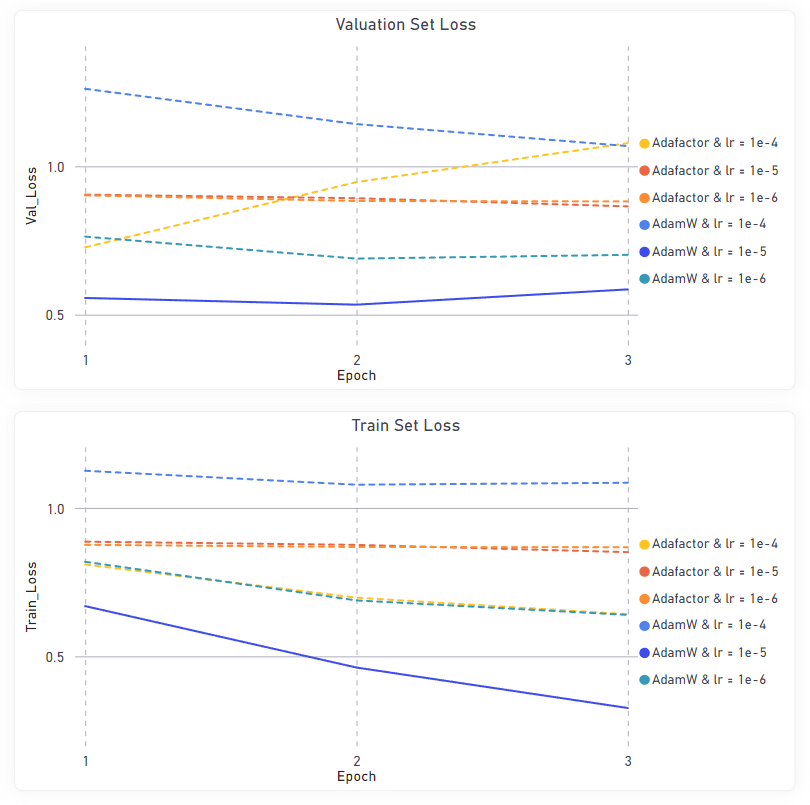
\includegraphics[width=\textwidth]{BERT_Loss.png}
    \caption{Loss of LSTM over epochs}
    \label{fig:BERT_Loss}
\end{figure}


\section{Discussion}

The 'to the moon' WallStreetBets movement had a tremendous impact on the lives of individuals, both to the positive and negative. 
Besides that, however, many investment funds have also been negatively impacted by the recent short-squeezes. 
While it might seem noble to root for individuals who try to force large funds out of their positions at big losses, it is easy to forget that many 
of those funds manage money for charitable endowments, pensions and others. 
Furthermore, such disruptions to the financial markets can harm its stability, thus causing spillover effects which can also negatively impact the 
lives of many people \citep{lyocsa2021yolotrading}.
By being able to accurately measure and monitor the sentiment on WallStreetBets, market participants and regulators are able to preemptively take measures.\\
However, since the wallstreetbets subreddit has become very popular just recently, there is little academic research about the impact of the community on 
financial markets so far. Even though there is some research about sentiment analysis on wallstreetbets, that research does not use state of the art algorithms to perform 
sentiment analysis. This thesis not only tries to shine some light on those new and influential market participants, but also tries to put forward some methods that work 
best to perform sentiment analysis on the forum. \\
Not only did this thesis compare the performance of different models, but also proposed a highly efficient and reliable way to create a domain-specific annotated corpus, 
which can be used as the input to aforementioned models. To my knowledge, this thesis is the first research that creates a domain-specific corpus for the WallStreetBets forum. 
Researchers, such as \cite{talamas2021socialmediaeffectsonthemarket}, specifically propose future work on “inclusion of features derived from alternative manipulation of the data like sentiment analysis 
could lead to new insights“. I strongly believe that the methods proposed in my thesis lead to better sentiment classifiers, 
which can then be used in other scientific or industrial applications.

\section{Conclusion}
This thesis proposes the use of an Active Learner to drastically reduce the total cost of annotation. 
As a result, it becomes more feasible to create a fully labeled domain-specific dataset. 
Once a fully labeled dataset is obtained, it can be used in supervised learning algorithms. 
The results show that using state of the art models underperform the simple baseline NB classifier.

\bibliography{references}


\end{document}